\chapter{Extension to two dimensions}\label{ch:joint2d}

The 1-D study keeps every target at the slant range of the reference point. In a real scene the terrain varies in range as
well, the residual $\Delta C_{0,i}$ depends on both coordinates, the echoes migrate in range and the range envelope of each channel is
shifted by half its path difference. A second simulator handles 3-D scenes with along- and cross-track baselines and
range-compressed data, and the joint reconstruction is extended to it.

\section{Model}

The unknown is the focused image $g[n,m]$ (\cref{fig:chain2d}) on azimuth positions $x_n$ (full PRF) and slant ranges of closest approach $r_m$.
The range-compressed data of channel $i$ are modelled as
\begin{equation}
  \bm s_i = \mathcal D\Bigl\{ K_i \cdot \mathcal F_r\bigl[\, Q_i \cdot \mathcal F_a( S_i\, g )\bigr] \Bigr\}
  \;+\; \text{(envelope term)},
\end{equation}
with
\begin{itemize}
  \item $S_i$, the terrain screen at every pixel, $\exp\bigl(-\jj 2\pi\Delta C_{0,i}(x,r)/\lambda\bigr)$, computed from the DEM in radar
        geometry (the ground range of each pixel is found by a fixed-point iteration, \cref{fig:demradar}, which converges for
        range slopes below $\tan\theta$, i.e.\ without layover);
  \item $Q_i(f;r)$, what changes with the range of closest approach in the range-Doppler domain: the azimuth chirp relative
        to the reference range and the differences of the coefficients $C_0,C_1,C_2,\Delta t$ of the channel;
  \item $K_i(f,f_r)$, the 2-D kernel: the 2-D FFT of the simulated echo of the reference point in channel $i$ at the full PRF
        (chirp, range migration, window of the pair, co-registration by $C_{0,i}/2$);
  \item the envelope term, the first-order shift of the range envelope by $\frac12[\Delta C_{0,i} + C_{0,i}(r)-C_{0,i}(r_\mathrm{ref})]$,
        valid while this shift is small compared with the range resolution.
\end{itemize}
\begin{figure}[htbp]
\centering
% DEM in radar geometry: the same slant range lands on another ground range when the terrain is high
\begin{tikzpicture}[x=1cm,y=1cm]
  \fill[terrainfill] (0,0) -- (0,0.25) .. controls (2.5,0.25) and (3.5,0.4) .. (4.6,1.25) .. controls (5.6,2.0) and (6.6,1.7) .. (8,1.2) -- (8,0) -- cycle;
  \draw[terrain,line width=0.9pt] (0,0.25) .. controls (2.5,0.25) and (3.5,0.4) .. (4.6,1.25) .. controls (5.6,2.0) and (6.6,1.7) .. (8,1.2);
  \draw[inkb,dashed] (0,0.25) -- (8,0.25) node[right,nota] {flat terrain};
  \node[sat] at (-1.2,4.6) {};
  \node[nota,above=2pt] at (-1.2,4.65) {platform (track into the page)};
  \draw[cblue,line width=0.8pt] (3.47,0.25) arc[start angle=-43.0,end angle=-30.5,radius=6.39];
  \draw[cblue,->] (-1.2,4.6) -- (4.25,0.95) node[midway,above,sloped,nota,text=cblue] {slant range $r$};
  \fill[cblue] (4.25,0.95) circle (2pt);
  \fill[inkb] (3.47,0.25) circle (2pt);
  \draw[cota] (3.47,-0.25) -- (4.25,-0.25) node[midway,below,nota] {same $r$, other $y$};
  \draw[inkb,densely dotted] (4.25,0.95) -- (4.25,-0.25); \draw[inkb,densely dotted] (3.47,0.25) -- (3.47,-0.25);
  \draw[cota] (4.75,0.25) -- (4.75,0.95) node[midway,right,nota] {$h$};
  \draw[->,inkb] (0,-0.95) -- (8,-0.95) node[right,nota] {ground range $y$};
\end{tikzpicture}

\caption[The DEM in radar geometry]{The DEM in radar geometry: a pixel at slant range $r$ lies on the terrain at another ground
range than on flat terrain. The ground range is found by the fixed-point iteration $y\leftarrow\sqrt{r^2-[H-h(x,y)]^2}$, which
contracts while the range slope stays below $\tan\theta$.}
\label{fig:demradar}
\end{figure}

\begin{figure}[htbp]
\centering
% Model of the 2-D joint reconstruction and its adjoint
\begin{tikzpicture}[x=1cm,y=1cm]
  \node[nota,anchor=west,text=ink] at (-0.9,1.25) {\textbf{model}: from the focused image to the range-compressed data of channel $i$};
  \node[opx] (g) at (0,0) {$g[n,m]$};
  \node[opx] (s) at (2.05,0) {$\times\,S_i$\\ relief};
  \node[opf] (fa) at (3.95,0) {$\mathcal F_a$};
  \node[opf] (q) at (5.85,0) {$\times\,Q_i$\\ per range};
  \node[opt] (fr) at (7.75,0) {$\mathcal F_r$};
  \node[opt] (k) at (9.65,0) {$\times\,K_i$\\ 2-D kernel};
  \node[opt] (d) at (11.55,0) {$\mathcal D$\\ decimate};
  \node[bdata,minimum height=9mm] (o) at (13.45,0) {$s_i[k,m]$};
  \foreach \a/\b in {g/s,s/fa,fa/q,q/fr,fr/k,k/d,d/o} \draw[seta] (\a) -- (\b);
  \draw[caqua,line width=2pt] (-0.6,-0.95) -- (2.95,-0.95) node[midway,below,nota,text=caqua!70!black]{azimuth $\times$ range};
  \draw[cblue,line width=2pt] (3.25,-0.95) -- (6.85,-0.95) node[midway,below,nota,text=cblue!85!black]{Doppler $\times$ range};
  \draw[corange,line width=2pt] (7.15,-0.95) -- (12.4,-0.95) node[midway,below,nota,text=corange!85!black]{Doppler $\times$ range frequency};
  \begin{scope}[yshift=-3.3cm]
  \node[nota,anchor=west,text=ink] at (-0.9,1.25) {\textbf{adjoint}: repeat the spectrum, 2-D matched filter, remove the relief, sum the channels};
  \node[bdata,minimum height=9mm] (o') at (0,0) {$s_i[k,m]$};
  \node[opt] (d') at (1.9,0) {$\mathcal D\Hm$\\ repeat};
  \node[opt] (k') at (3.8,0) {$\times\,K_i^{*}$};
  \node[opt] (fr') at (5.7,0) {$\mathcal F_r^{-1}$};
  \node[opf] (q') at (7.6,0) {$\times\,Q_i^{*}$};
  \node[opf] (fa') at (9.5,0) {$\mathcal F_a^{-1}$};
  \node[opx] (s') at (11.4,0) {$\times\,S_i^{*}$};
  \node[opx] (sum) at (13.3,0) {$\sum_i$};
  \foreach \a/\b in {o'/d',d'/k',k'/fr',fr'/q',q'/fa',fa'/s',s'/sum} \draw[seta] (\a) -- (\b);
  \node[nota,below=1.5mm of k'] {RCMC, azimuth\\ compression,\\ co-registration};
  \end{scope}
\end{tikzpicture}

\caption[The model of the 2-D joint reconstruction]{The model of the 2-D joint reconstruction and its adjoint (the envelope
term is omitted). The relief acts per pixel, the range-dependent focusing per range line in the range-Doppler domain, and the
2-D kernel of the channel in the two-dimensional frequency domain.}
\label{fig:chain2d}
\end{figure}

The image is kept on a range grid twice as fine as the data, because a phase that varies with range shifts the range spectrum.
The adjoint passes the adjoint test to $2.6\times10^{-7}$; the solver is the same CGLS as in 1-D ($\mu=0.03\,\sigma_{\max}$,
two passes of up to 60 iterations).

\section{The common range band}

A cross-track baseline shifts the range spectrum seen by the channel, the spectral shift known from interferometry:
\begin{equation}
  \nu_i = \frac{c\,\bxt_{,i}\cos\theta}{2\lambda\, r\tan(\theta-\alpha)},
\end{equation}
with $\alpha$ the range slope of the terrain; on flat terrain this is \SI{0.202}{MHz} per \SI{100}{m} of baseline. Range
frequencies that only some channels observe are not determined by the data (fewer equations than folded parcels), and the
joint reconstruction leaves the full ambiguity there. In a control case (one target, flat terrain, $\bxt=[0,300,119.8,100.5]$\,\si{m},
exact model) the full band reaches \SI{-40.5}{dB}, whereas the band common to all four channels reaches \SI{-66.1}{dB}, equal to
the reference in the same band. The output is therefore limited, pixel by pixel, to the range frequencies that every channel
observes there, and the reference and the uncorrected reconstruction are compared in the same band. The price is range
resolution, a fraction $\bxt/\bxt^{\mathrm{crit}}$ of the band; with the \SI{5}{MHz} bandwidth of the sweeps the median pixel
keeps \SI{93}{\percent} of the band and the worst pixel \SI{45}{\percent}. A wider system bandwidth (e.g.\ \SI{50}{MHz})
would reduce this loss about tenfold.

\Cref{fig:example2d} shows a 3-D case: 49 targets on an isolated \SI{1000}{m} mountain with four channels and
$\bxt^{\max}=\SI{300}{m}$.

\begin{figure}[p]
\centering
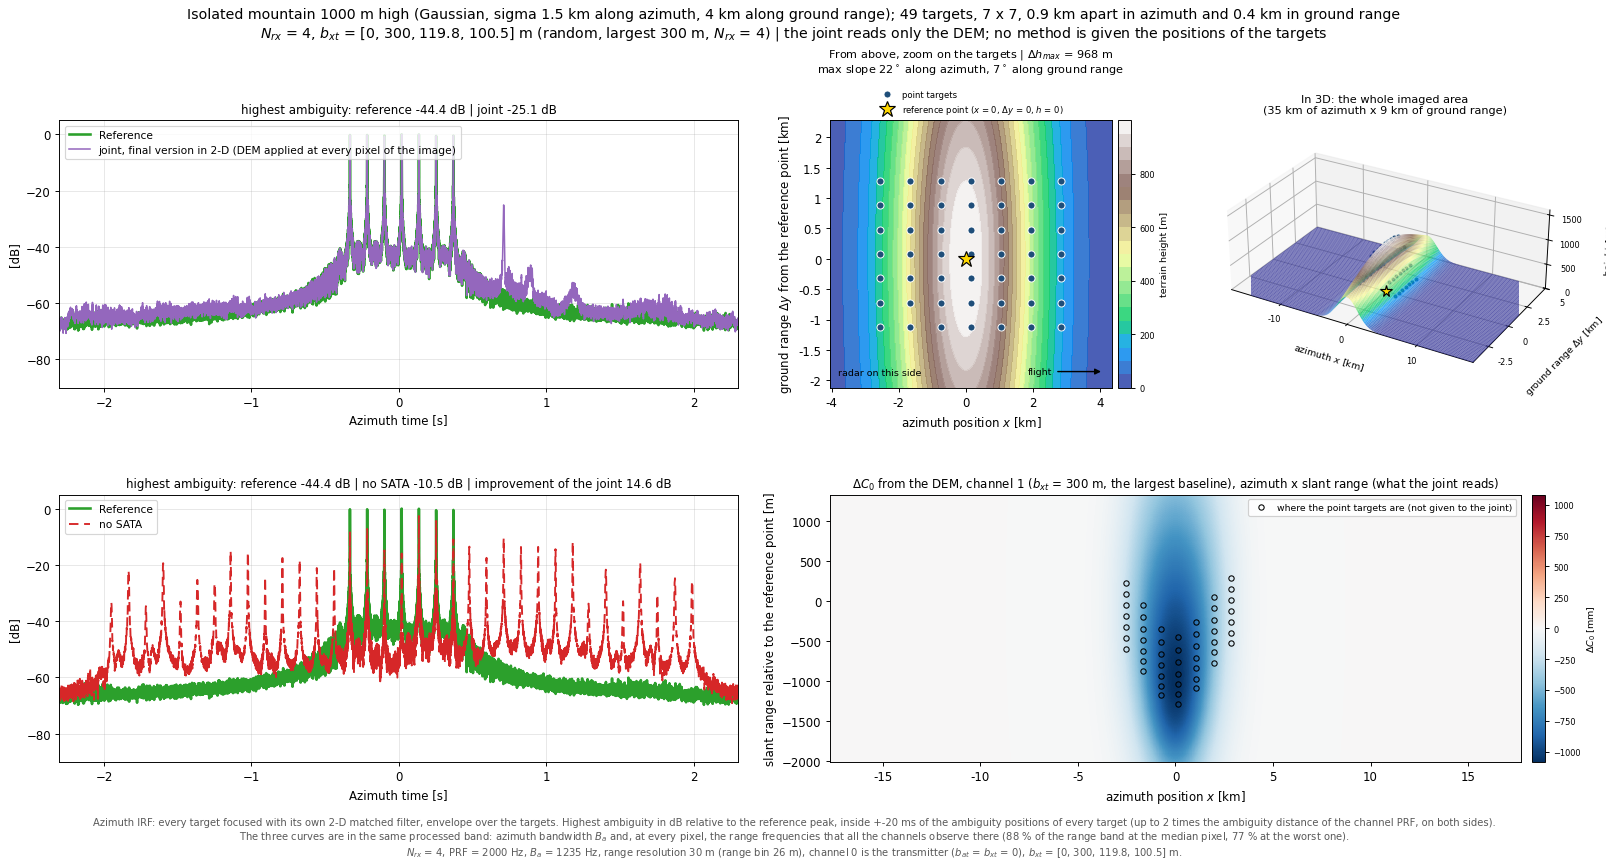
\includegraphics[width=\linewidth]{figures/sweep2d_mountain49_N4b300.png}
\caption[Example of the 2-D sweep]{A page of the 2-D sweep: 49 targets on an isolated \SI{1000}{m} mountain (Gaussian,
$\sigma=\SI{1.5}{km}$ in azimuth and \SI{4}{km} in ground range), $\Nrx=4$, $\bxt=[0,300,119.8,100.5]$\,\si{m}. Top left:
reference and joint reconstruction; bottom left: reference and no correction; right: the scene and the $\dC$ of the channel
with the largest baseline, which is all the joint reconstruction reads. This is one of the harder cases (the joint
reconstruction leaves \SI{-25.1}{dB}, an improvement of \SI{14.6}{dB}).}
\label{fig:example2d}
\end{figure}
